\chapter{Quem cai primeiro}\label{cap:primeiro}

O capítulo anterior mediu a direção do tempo dentro de uma série. Falta a mesma pergunta no par:
quando as coisas ruins vêm juntas, alguém cai primeiro, e essa ordem se repete?

\section{A ordem que a proteção supõe}

O índice americano e o Ibovespa caem juntos muito mais do que a independência prevê ---
\numConjuntaExcesso{} vezes, medidos nos \numConjuntaDias{} dias em que as duas séries têm corte, com
\numConjuntaRompeA{} rompimentos de um lado, \numConjuntaRompeB{} do outro e \numConjuntaJuntos{} dias
em que os dois rompem ---, e \numConjuntaAcompanhados{} dos rompimentos de uma perna vêm com a outra
no mesmo dia. A leitura
natural de um número desses é que a queda conjunta é um acontecimento só, sem ordem interna: o dia
de uma perna encontra o dia da outra e pronto.

Se for assim, proteger uma perna não ajuda a outra nem atrapalha, porque não há intervalo entre as
duas quedas para fazer nada. A pergunta é se esse intervalo existe.

\section{A contagem}

O instrumento é uma contagem de episódios, e a regra precisa ser dita antes de ser usada.

% aterramento: episodio
\begin{definicao}[episódio dirigido]\label{def:episodio}
Um \emph{episódio} começa no dia em que uma das pernas rompe o próprio corte, desde que nenhum
episódio tenha começado nos \numConjuntaJanelaEpisodio{} dias anteriores --- rompimentos dentro
desses dias não abrem episódio novo. O episódio é \emph{dirigido} quando a outra perna rompe dentro
dos mesmos \numConjuntaJanelaEpisodio{} dias seguintes, e a perna que rompeu primeiro é a
\emph{líder}. A \emph{assimetria} é a diferença entre os episódios liderados por uma perna e os
liderados pela outra, dividida pelo total de episódios dirigidos.
\end{definicao}

Vale um exemplo, porque esta é a única regra do capítulo. Se uma perna rompe num dia e a outra rompe
quatro dias depois, o primeiro rompimento abre o episódio, o segundo o torna dirigido, e a perna que
rompeu primeiro é a líder --- e o segundo rompimento, por cair dentro dos
\numConjuntaJanelaEpisodio{} dias de um episódio que já começou, não abre episódio nenhum.

A regra tem um viés próprio, e escondê-lo seria medir a regra em vez do mundo: a espera olha para
trás e a detecção olha para a frente, de modo que num par sem adiantamento nenhum os dois lados não
saem iguais. Por isso o número do par real só vale contra o número dos pares sorteados, e nunca
contra zero --- é a mesma disciplina dos capítulos do orçamento e da direção.

Pelo mesmo motivo a inversão do relógio não serve de conferência aqui. No capítulo da direção ela
funcionou, porque a estatística de lá não tinha regra nenhuma dentro; aqui a regra é assimétrica, e
virar o mundo ao contrário não a vira junto. Quem confere este instrumento é o nulo, que carrega a
mesma regra.

\section{O nulo, e o par}

Medindo \numConjuntaNulos{} pares sorteados e contemporâneos com a mesma regra, a assimetria tem
média \numConjuntaNuloMedia{} e dispersão \numConjuntaNuloDispersao{}. A média é praticamente zero. Um dia em que as duas caem juntas não tem
primeiro.

Contra esse nulo, o par como veio faz o seguinte.

\begin{table}[htbp]
  \centering
  \small
  \resizebox{\linewidth}{!}{%
\begin{tabular}{rrrr}
    \hline
    janela do & episódios & episódios & assimetria \\
    episódio & liderados pelo índice & liderados pelo Ibovespa & medida \\
    \hline
    um & \numConjuntaLiderAUm & \numConjuntaLiderBUm & \numConjuntaAssimetriaUm \\
    cinco & \numConjuntaLiderACinco & \numConjuntaLiderBCinco & \numConjuntaAssimetriaCinco \\
    dez & \numConjuntaLiderADez & \numConjuntaLiderBDez & \numConjuntaAssimetriaDez \\
    vinte e um & \numConjuntaLiderAVinteEUm & \numConjuntaLiderBVinteEUm & \numConjuntaAssimetriaVinteEUm \\
    \hline
  \end{tabular}}
  \caption{Os episódios dirigidos no par, por janela. A janela é quanto tempo se espera pela
    segunda perna depois de a primeira ter rompido.}
  \label{tab:episodios}
\end{table}

Na janela de \numConjuntaJanelaEpisodio{} dias o índice lidera \numConjuntaLiderA{} episódios e o
Ibovespa lidera \numConjuntaLiderB{}, o que dá uma assimetria de \numConjuntaAssimetria{} ---
\numConjuntaDesvios{} desvios acima do nulo. O número é positivo em todas as janelas testadas, e
não é pequeno.

\section{Quanto dura o adiantamento}

A assimetria diz que existe uma ordem; ela não diz de quanto tempo é o intervalo. Para medir isso, o
instrumento é posto à prova contra um adiantamento declarado: a segunda perna é deslocada dia a dia
e a assimetria é remedida.

\begin{figure}[htbp]
  \centering
  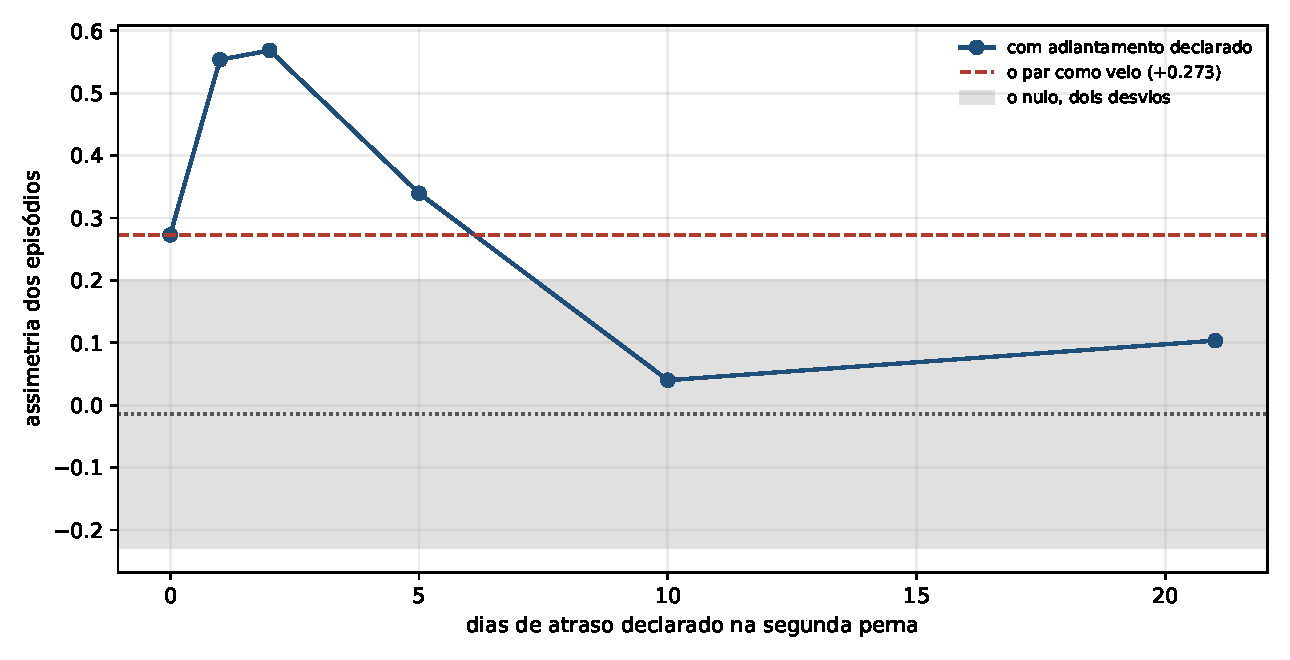
\includegraphics[width=\linewidth]{figuras/E14_direcao_conjunta_1.pdf}
  \caption{A assimetria contra o atraso declarado na segunda perna. A faixa cinza é o nulo a dois
    desvios \emph{sem} deslocamento, a linha tracejada é o par como veio, e a curva é o par com o
    atraso declarado --- que o nulo também sofre, e é o que o texto mede.}
  \label{fig:adiantamento}
\end{figure}

A curva sobe antes de descer. Sem deslocamento nenhum a assimetria é \numConjuntaControleZero{}.
Com a segunda perna deslocada em um ou dois dias, ela chega ao seu máximo ---
\numConjuntaControleUm{} e \numConjuntaControleDois{} ---, acima do valor do par como veio. Com
cinco dias cai para \numConjuntaControleCinco{}, com dez dias para \numConjuntaControleDez{}, e com
\numConjuntaAtrasoMaior{} dias para \numConjuntaControleVinteEUm{}, dentro da faixa do nulo.

Mas o nulo sobe junto, e é isso que a subida mede. Aplicando aos pares sorteados o \emph{mesmo}
deslocamento declarado, a assimetria do nulo no atraso de um dia vale
\numConjuntaNuloDeslocadoUm, contra \numConjuntaNuloDeslocadoZero{} sem deslocamento nenhum: um par
que não tem adiantamento algum pica no mesmo lugar, e o pico é do instrumento.

Vale dizer o que o eixo faz. Os seis pontos estão na posição do atraso que declaram, de modo que o
passo de dez para vinte e um dias ocupa onze vezes a largura do passo de zero para um. O pico cai no
trecho mais estreito do desenho: quem olha a curva de longe vê um tremor no começo da linha, e é ali
que está o achado.

O que a varredura localiza é menos do que a subida sugere. Contra o nulo deslocado, a evidência do
par no atraso zero é de \numConjuntaDesvios{} desvios, e nos atrasos de um e dois dias ela fica da
mesma ordem --- \textbf{o que esta medição sustenta é que existe uma ordem, e num intervalo curto;
ela não separa um dia de dois}. O intervalo curto é o que uma proteção teria entre o rompimento de
uma perna e o da outra, e é ele que decide se há alguma coisa a fazer no meio.

\section{Se repete}

Uma direção medida uma vez é um episódio do dado, e não uma propriedade dele. A conferência é
partir o par em pedaços e medir cada um.

\begin{figure}[htbp]
  \centering
  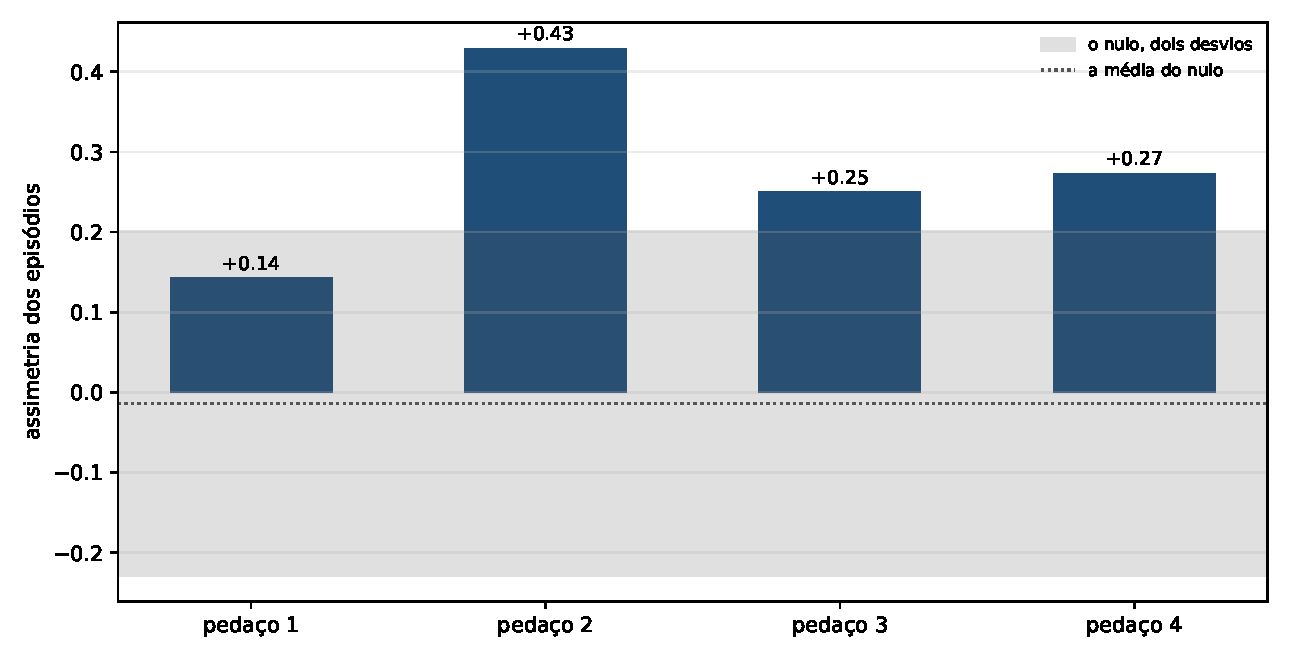
\includegraphics[width=\linewidth]{figuras/E14_direcao_conjunta_2.pdf}
  \caption{A assimetria em cada pedaço do par, contra a faixa do nulo. Os quatro pedaços do par têm
    \numConjuntaPrimeiroDias{}, \numConjuntaSegundoDias{}, \numConjuntaTerceiroDias{} e
    \numConjuntaQuartoDias{} dias de série, e o primeiro perde a janela inicial, em que o corte
    ainda não existe.}
  \label{fig:pedacos}
\end{figure}

Os quatro pedaços dão \numConjuntaPrimeiroAssimetria{}, \numConjuntaSegundoAssimetria{},
\numConjuntaTerceiroAssimetria{} e \numConjuntaQuartoAssimetria{}: todos positivos, e
\numConjuntaPedacosAcima{} de \numConjuntaPedacos{} acima da média do nulo. O sinal se repete --- com
uma ressalva que a régua certa impõe: medida no comprimento de \emph{um} pedaço, a faixa do nulo tem
dispersão de \numConjuntaNuloPedacoDispersao{} e borda de dois desvios em \numConjuntaNuloPedacoBorda,
e nenhum pedaço sozinho a alcança. O que se repete é o sinal, não a evidência de cada pedaço. O
tamanho varia bastante de pedaço para pedaço, e o motivo está na contagem: os quatro pedaços têm
\numConjuntaPrimeiroLiderA{}, \numConjuntaSegundoLiderA{}, \numConjuntaTerceiroLiderA{} e
\numConjuntaQuartoLiderA{} episódios dirigidos liderados pelo índice, e com tão poucos episódios cada
pedaço, sozinho, não distingue nada.

\section{O que fica}

Fica a resposta da travessia, e ela é um sim com medida. A perda conjunta tem direção: o índice cai
primeiro, o Ibovespa vem atrás no intervalo curto que a varredura delimita, e a ordem se repete nos
quatro pedaços do dado. A precisão fica de fora. O efeito é de \numConjuntaDesvios{} desvios sobre o total do
par, cada pedaço isolado é fraco, e a regra de contagem não pode ser conferida pelo relógio
invertido, porque a regra ela mesma tem lado.

Fica também o que a travessia inteira mostrou, olhando para trás. Cinco perguntas medidas com o
instrumento de outra família, e as cinco deram o mesmo tipo de resposta: existe sinal, e o sinal
custa --- em dias de experimento, em trabalho de atualização, em passado apagado, em anos de espera.
Cada capítulo desta travessia terminou com um preço medido, e onde a conta prometeu o que o mundo
não pagou --- como no vigia da direção --- o preço ficou declarado em vez de escondido.

O que sobra é a pergunta que a travessia deixa de pé ao terminar. Quase tudo o que a espiral mediu
até aqui se compra: memória se compra com dias, atualização se compra com trabalho, um experimento
se compra com replicatas. A espiral vira agora para o outro lado da mesma conta, e a pergunta do
movimento seguinte é o que \textbf{não} se compra de jeito nenhum --- começando pela mais dura de todas,
que é o mundo que não foi observado.
